%--------------------------------------------------------------
% Eliot Aretskin-Hariton
%-------------------------------------------------------------
\documentclass[]{NASA}

% List of authors with affiliation for the cover page
\AuthorAffiliation{Eliot D. Aretskin-Hariton\\ 
  Glenn Research Center, Cleveland, Ohio\\[10pt] 
  Ghost Writer\\
  Glenn Research Center, Cleveland, Ohio\\[10pt] 
  Arthur Dent\\                                          
  Megadodo Publications, Islington, London\\[10pt]
  }
\NasaCenter{Glenn Research Center\\Cleveland, Ohio 44135}
\Type{TM}                    % TM, TP, CR, CP, SP, TT
\SubjectCategory{xx}         % two digit number
\LNumber{xxxxx}              % Langley L-number
\Number{YOURTMNUMBERGOESHERE}              % TM Report number
\Month{04}                   % two digit number
\Year{2022}                  % four digit number
\SubjectTerms{overleaf, editing}     % 4-5 comma separated words
\Pages{tbd}                   % all the pages from the front to back covers
\DatesCovered{04/2022--}              % 10/2000--9/2002
\ContractNumber{}            % NAS1-12345
\GrantNumber{}               % NAG1-1234
\ProgramElementNumber{}
\ProjectNumber{}             % NCC1-123
\TaskNumber{}                % Task 123
\WorkUnitNumber{}            % 123-45-67-89
\SupplementaryNotes{}

\Acknowledgment{Describe who funded your effort, which organizations, and which Research Center. For Example: Funding for the effort was provided under the directed guidance of the Heart-of-Gold Project by Project Manager Zaphod Beeblebrox of the Magrithean Research Center.}

\abstract{
\hspace{\parindent}This guide is meant to help NASA authors to quickly format \ac{TM} for publishing. This document is intended for use with Overleaf, a web-based collaborative document writing program. We will show you some examples of how to write \LaTeX ~to make figures, automatically create references, make tables, and many other useful things that you will need for your \ac{TM}. 
}

% Title, Author
%-------------------------------------------------------------
\title{A Technical Memorandum Template Example for use with Overleaf}

\author{
  Eliot Aretskin-Hariton and Ghost Writer\\
  National Aeronautics and Space Administration\\
  Glenn Research Center\\
  Cleveland, Ohio 44135\\
  \vspace{5mm}
  Arthur Dent\\
  Megadodo Publications\\
  Islington, London\\
  }


%-------------------------------------------------------------
\begin{document}
\maketitle
\newpage

%% ----------------------------------------------------------------------------------------------------------------------------------------
%% 										 Nomenclature
%% ----------------------------------------------------------------------------------------------------------------------------------------
\section*{Nomenclature}
\subsection*{Acronyms}
\begin{tabbing}
%  \hspace{0.45\linewidth}\textit{Acronyms} \\
  XXXXXXXXXXXXX \= \kill% this line sets tab stop
  \acs{ASAP} \> \acl{ASAP} \\
  \acs{ANA} \> \acl{ANA} \\
  \acs{PR} \> \acl{PR} \\
  \acs{TM} \> \acl{TM} \\
  \acs{WYSIWYG} \> \acl{WYSIWYG} \\

\end{tabbing}

\subsection*{Variables}
\begin{tabbing}
%  \hspace{0.45\linewidth}\textit{Acronyms} \\
  XXXXXXXXXXXXX \= \kill% this line sets tab stop
  $b$ \> a new variable (kg) \\
  $GS15$ \> the grade you wish to attain at NASA \\
  $m$   \> some other variable (kg/s) \\
  $x$ \> some other variable (s) \\
  $y_1$ \> some variable (kg) \\ 
  $y_2$ \> a final variable ($s^2/kg$) \\
\end{tabbing}
\acresetall         % Force reset of all acronyms (from intro and list)

% Create the Acronym List
% For ease of updating, add acronyms alphabetical by acronym
% Brought to you by the letter "C"  =][
%
  \begin{acronym}

    % The Letter A
    \acro{ASAP}{as soon as possible}
    \acro{ANA}{a new acronym}
    \acro{AOA}{angle of attack}
    \acro{ANOPP2}{Aircraft NOise Prediction Program 2}

    % The Letter B
    

    % The Letter C
    % Brought to you by the letter 'C'.  'C' is for Cookie
	 \acro{CNT}{carbon nanotube}
	 \acro{CCBlade}{Continuity and Convergence Blade}
	 \acro{CCE-LIMX}{Combined Cycle Engine Large-Scale Inlet for Mode Transition Experiments}

    % the letter D
     \acro{DYMOS}{DYMOS}
     \acro{DMRJ}{dual-mode ramjet}
    % The Letter E

     
    % The Letter F

     
    % The Letter G
    
    % The Letter H
     \acro{HSFP}{high-speed airflow path}
     \acro{HS-MFP}{high-speed mass flow plug}
     \acro{HSC}{high-speed cowl}

    % The Letter I
    \acro{IPR}{isolator pressure ratio}

    % The Letter L
    \acro{LSC}{low-speed cowl}

    % The Letter M 
     \acro{MTO}{maximum takeoff weight}
     \acro{MFP}{mass flow plug}

    % The Letter N


    % The Letter O
     \acro{OMDAO}{Open Multidisciplinary Design Analysis and Optimization}
     \acro{OAS}{Open Aero Struct}
     \acro{OBEMT}{Open Blade Element Momentum Theory}

    % The Letter P
    \acro{PR}{pull request}
     \acro{PVD}{physical vapor deposition}
     \acro{pyCycle}{pyCycle}

    % The Letter R


    % The Letter S
    \acro{SWT}{10- by 10-Foot Supersonic Wind Tunnel}

    
    % The Letter T
    \acro{TM}{technical memorandum}
    \acro{TTT}{Transformative Tools and Technologies}
    \acro{TMS}{Thermal Management System}
    \acro{TBCC}{turbine-based combined cycle}
     
    % The Letter U
     \acro{UAM}{Urban Air Mobility}
     
    % The Letter V
     \acro{VTOL}{Vertical Take-off and Landing}
    % The Letter W
    \acro{WYSIWYG}{what you see is what you get}

	% The Letter X
	 \acro{XDSM}{eXtended Design Structure Matrix}
	
	% The letter Z
	 \acro{Zappy}{Zappy}

  \end{acronym}
%    % Input the full acronym list

%\tableofcontents

% ============================================================================================
% ============================================================================================

\newpage
\section{Introduction} \label{sec:Introduction}
\begin{flushleft} % This changed the document from justify to raggedright
\setlength{\parindent}{20pt}

\hspace{\parindent} This document is a template to assist you in creating a new \ac{TM} per the NASA style guide. 
You can start with this document and insert your own text and figures, following the examples we have provided. 
This should save you considerable time when preparing your document for publication. 
The document is a general guide and will provide you a number of basic tools like figure and table creation, automatic handling of acronyms, bibliography examples, and how to reference different sections of the paper. 
If you see errors or inaccuracies you are encouraged to make changes and submit a \ac{PR} to the GitHub repository\footnote{\url{https://github.com/ehariton/TM_template}}. 
Please note that this document is a work in progress and no organization has yet expressed interest in funding this effort. 

The history of what has come before is important to include in any document. So I am going to talk a little about the history of \LaTeX ~at NASA. 
NASA up to this point has had little focus on using \LaTeX. While individual researchers often used it, generally collaborative document writing was done in word via email. 
In 2009, Bill Wood and Bil Kleb wrote the original \emph{NASA.cls} style, which this document is based on. Aaron Swank of NASA GRC made some edits since that time. 
Most recently, in 2022, Eliot Aretskin-Hariton made some modifications the style document in an attempt to make the document better match the NASA GRC style requirements levied on him by the unrelenting NASA editing department. 
The result, after being stripped of any useful technical material, is the document you are reading right now. 

Writing style is very important. While writing any technical document, I encourage you to use the \emph{general-to-specific} writing style. 
This style focuses on talking about general things first, and then slowly narrowing down your focus to talk about specific things. 
This is why we started talking about the history of \LaTeX ~at NASA before talking about our thesis sentence. 
This style should be generally applied to sections, as well as individual paragraphs themselves. 
Notice how we started this paragraph with the words \emph{"Writing style"}. We are trying to let any reader that is quickly skimming the document, that this paragraph is about style, and thus can safely be ignored if the reader is searching for something else. 
I could have started this paragraph with the phrase \emph{"Some comments about writing style"}. 
However, this is slower for the reader to parse because they keywords \emph{"writing style"} only appear at the end of the sentence. 

Everyone in the world is busy, they do not want to read your document from start to end. 
They want to skim it, pull out the most relevant information as quickly as possible, and then get on with the rest of their life. 
Think about how you read documents. 
Do you read every technical document start to finish? 
Did you skip over paragraphs? 
Did you skip over this paragraph? 
It is very possible because there is a wall of text and you have not seen any figures yet. 
Your goal as a writer should be to enable speedy and clear transfer of information from your text to their brain. 
You can accomplish this by following the \emph{general-to-specific} writing style.

The goal of this document is included in the thesis sentence that you are about to read. 
I mentioned the keyword \emph{goal} at the start of the previous sentence to let readers know that the thesis is contained in this paragraph. 
The purpose of this document is to enable faster and more-efficient collaborative document writing for the NASA community, without all the mucking-about using word processors, email, and other unspeakable horrors. 
In this document I will endeavor to give you plenty of examples to satiate your technical desires, with the hope that we can all publish better papers faster. 
This should lead to speedy promotions and more time to spend doing constructive things like trying to understand why finite differencing is such a terrible way to get derivatives of a function.

At the end of your introduction you always want to tell the reader what they are going to read about in the remainder of the document. 
This means you need to reference other sections of the document. 
To do this that section needs a label, which you can view in the source \emph{main.tex} document. 
Then you can reference the label in-line with the text as is shown in the next paragraph.

The remainder of the report is organized as follows: 
Section~\ref{sec:methods} will talk about the different methods you can use to do interesting things like make figures, how to use acronyms, and how to insert citations.
Following that, Section~\ref{sec:results} is a placeholder where you can enter in the results of your paper.
Finally, conclusions of the work will be presented in Section~\ref{sec:Conclusion}.

% ================= A SECTION SEPARATOR IS USEFUL FOR WHEN YOU ARE SCROLLING UP AND DOWN THE DOCUMENT =================
% ============================================================================================

\section{Methods to Make Useful Things} 
\label{sec:methods} 
This is a little introduction into what this section is about. Remember, you want to follow the \emph{general-to-specific} writing style that we talked about in Section \ref{sec:Introduction}. Give readers a little introduction to what this subsection contains. There is cool stuff in here I promise! Just keep reading and you will not regret spending your time with me. Please get me more downloads so I can get to $GS15$ \ac{ASAP}.

The underlying code that makes \LaTeX ~work is relatively straightforward combination of plain-text and a simple scripting language. One of the best learning resources for this language is the Overleaf help page\footnote{\url{https://www.overleaf.com/learn}}. We have included many examples throughout this document. To learn how to make your own ~\ac{TM}, simply open this document in Overleaf, and start editing the \emph{main.tex} file. 
This will open up the source code as well as the final pdf that you are reading now.
As we go through the next sections, scroll through both the source and the pdf to learn how to create these effects in your own document. 

Now that we are done with the formalities, we should tell the reader what is going to happen in the rest of the subsections. If I do not tell them these things they will get lost in the maze of text you am writing.
Subsection ~\ref{sec:subsections_exampel} will teach you how to make subsections. Subsection~\ref{sec:acronyms} will teach you how to deal with acronyms. Subsection~\ref{sec:equations} will show you how to make equations.
Subsection~\ref{sec:figures} will demonstrate how to include figures in the document.
Subsection~\ref{sec:tables} will demonstrate how to include tables in the document.
Subsection~\ref{sec:lists} will show you how to make lists.
And lastly, subsection~\ref{sec:citations} will demonstrate how to insert citations and a bibliography.

% ===============SUBSECTION SEPARATORS CAN BE FUN TOO ================= 
\subsection{A Subsection}
\label{sec:subsections_exampel}
Subsections are made like this. You can also give them labels so that you can reference them later. Referencing subsections is easy and you can see an example in Section~\ref{sec:subsections_exampel}. Subsection~\ref{sec:figures} will show you how to make figures large and small.

% ============================================================================================
\subsection{Acronyms}
\label{sec:acronyms}
You may have noticed that there is a \textit{acronyms.tex} file. This file holds all the acronyms that we will use in the paper. This allows us to reference acronyms we have already used (e.g. \ac{TM}) as well as \ac{ANA}. The document remembers where your first use an acronym and puts the whole explanation of the acronym in there. Upon your next usage in the paper, the acronym is abbreviated as normal just like \ac{ANA}. 

The Nomenclature is included on it's own page near the beginning of the document. The reasoning behind this is to allow readers of the document to print out this single page and have it alongside them as they read the rest of the document. That way any acronyms or variables that they have forgotten are easily and quickly looked-up. This is especially important when acronym and variable lists are large. Remember while you may remember all your acronyms, someone reading your document for the first, second, or even third time, has also read a hundred other documents with similar acronyms. Make like easy for them by leaving the Nomenclature on a separate page.
% ============================================================================================
\subsection{Equations}
\label{sec:equations}
Writing equations in-line with text is pretty easy. Just follow this example by adding \$ \$ around anything you want to be rendered as an equation: $\dot{w}_f$. You can also include equations as separate entities and even reference them later like  Equation~(\ref{eq:phi_basic}) and (\ref{eq:second_equation}).
\begin{equation}
\label{eq:phi_basic}
    y_1 = m \cdot x + b 
\end{equation}

\begin{equation}
\label{eq:second_equation}
    y_2 = \frac{x^2}{y_1 + 7}
\end{equation}

% ============================================================================================
\subsection{Tables}
\label{sec:tables}
Tables are a fantastically useful way of clearly showing information, or hopelessly confusing the reader. I try to avoid the latter generally speaking. Let me shown you an example of a Table~\ref{tab:step}. Note that the table won't necessarily show up exactly in the spot you expect.
\begin{table}[!tbph]
        \small
	\centering
	\caption{\raggedright{Actuator Characteristic Step Response. Variables are described in the Nomenclature.}}
	% head note goes here
	\begin{tabular}{ c | c | c | c }
	    \hline
	    Test & x & $y_1$ & $y_2$ \\
        & s & kg & $s^2/kg$ \\
		\hline
		\hline
		1 & 20.0 & 3.72 & 0.09 \\
        2 & -12.0	& 34.585  & 09 \\
        \hline
	\end{tabular}
	\label{tab:step}
\end{table}

% ============================================================================================
\subsection{Lists}
\label{sec:lists}
Sometimes we want to include lists of things in documents as well. Here I am going to write a list of why Overleaf is great:
\begin{enumerate}
  \item Collaborate with your colleagues to write awesome documents.
  \item No software download required.
  \item When 95\% of the formatting is taken care of, you can write documents faster.
  \item NASA editing department doesn't have to spend all their time correcting how you write lists. 
  \item The truth is that \ac{WYSIWYG} is overrated because of the manual work required to enforce formatting. 
\end{enumerate}

% ============================================================================================
\subsection{Figures}
\label{sec:figures}
If you want to display figures, you can use the example here to show a single figure and automatically reference it. 
Figure~\ref{fig:fd_is_terrible} is a great example of this. 
Many formats of figure files are acceptible including \emph{.pdf}, \emph{.eps}, and \emph{.png}. 
Please note, the figure will not necessarily show up in-line with the text, it may be automatically pushed to the end of the document. 
There are also neat side-by-side figures. 
We have an example of those in Figures~\ref{fig:baseline} and ~\ref{fig:advanced}. These figures show how to make independent side-by-side figures using minipage.
Side-by-side figures can also be made as sub-figures as shown in Figure ~\ref{fig:star_tracker}. We can also reference the individual sub-figures if we want to just talk about Figure~\ref{fig:baseline2} or Figure~\ref{fig:advanced2}.
If you have large figures that you want to show sideways, Figure~\ref{fig:optical_com} is a good example of how to do this.
\begin{figure}[bth]
  \centering
  \includegraphics[width=0.6\textwidth]{fd_is_terrible.png} \\
  \caption{\raggedright{Finite differencing noisy functions can lead you to just get wrong derivatives, depending on how large your step-size is.~\cite{Martins2021} Pro-tip, use complex step if you can.}}
  \label{fig:fd_is_terrible}
\end{figure}

\begin{figure}[!tbph]
  \centering
  \begin{minipage}{.45\textwidth}
  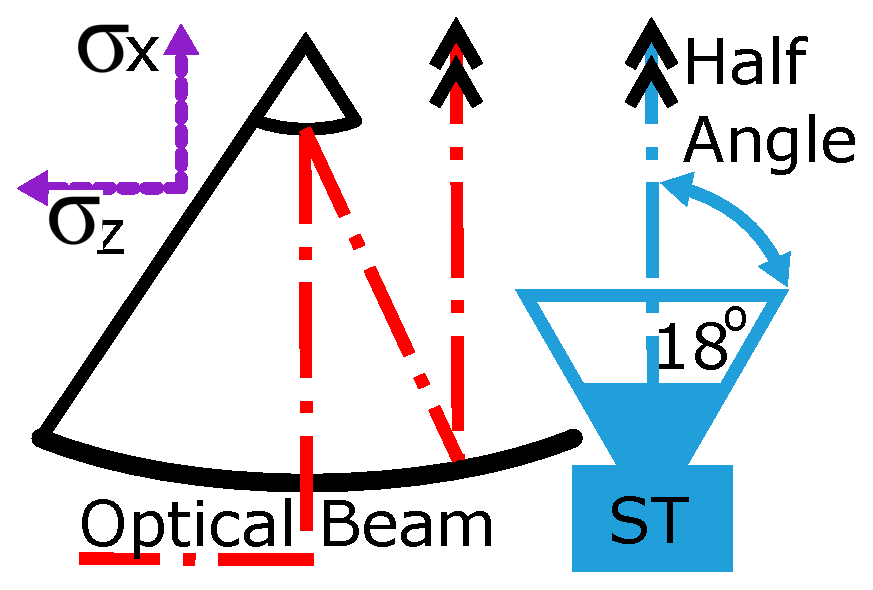
\includegraphics[width=1\linewidth]{figure1of4.eps}
  \caption{\raggedright{Baseline co-boresight configuration for star tracker.}}
  \label{fig:baseline}
  \end{minipage}
  \begin{minipage}{.02\textwidth}
  % add some space between figs
  \end{minipage}
  \begin{minipage}{.45\textwidth}
  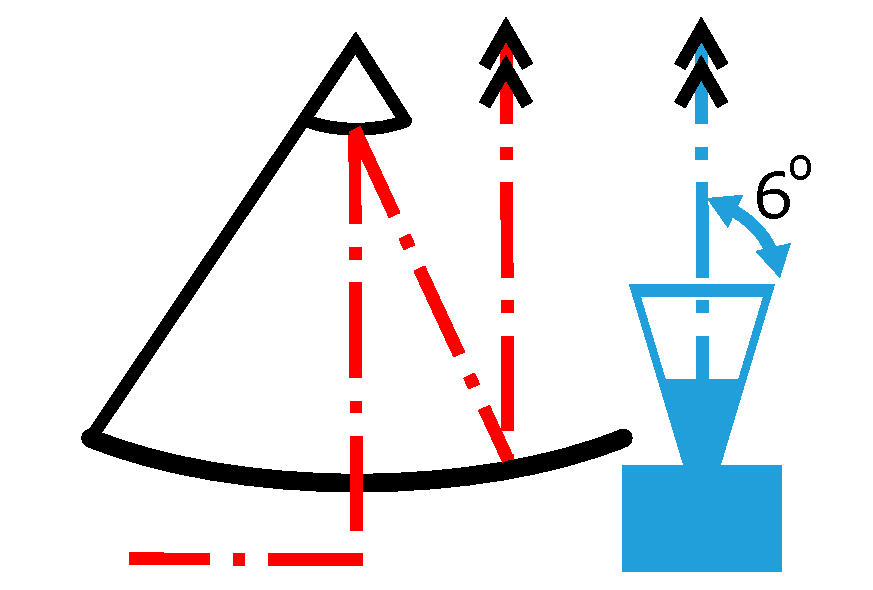
\includegraphics[width=1\linewidth]{figure2of4.eps}
  \caption{\raggedright{Advanced co-boresight configuration for advanced star tracker.}}
  \label{fig:advanced}
  \end{minipage}
\end{figure}

\begin{figure}[!tbph]
  \centering
  \subfloat[][\raggedright{Baseline co-boresight}]{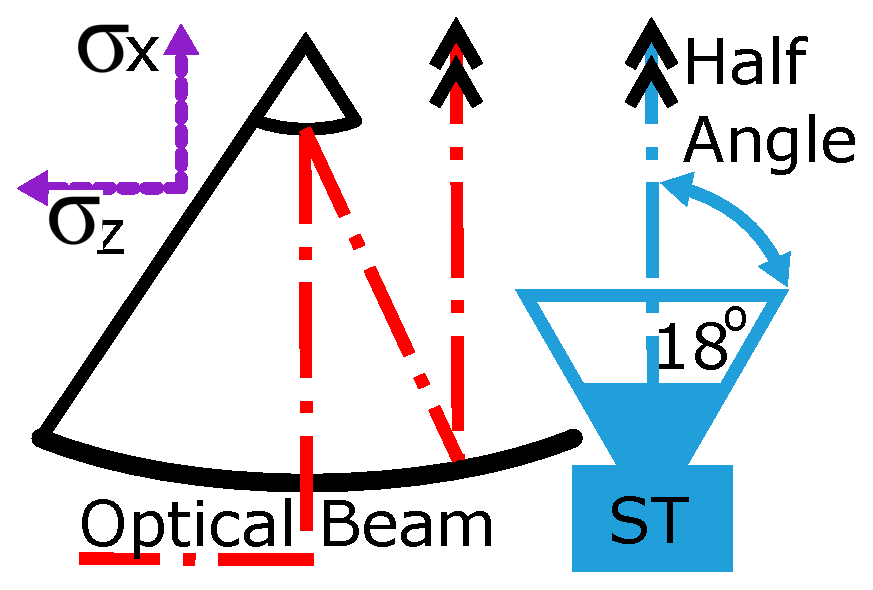
\includegraphics[width=0.45\linewidth]{figure1of4.eps}\label{fig:baseline2}}
  \hspace{0.5cm}
  \subfloat[][\raggedright{Advanced co-boresight}]{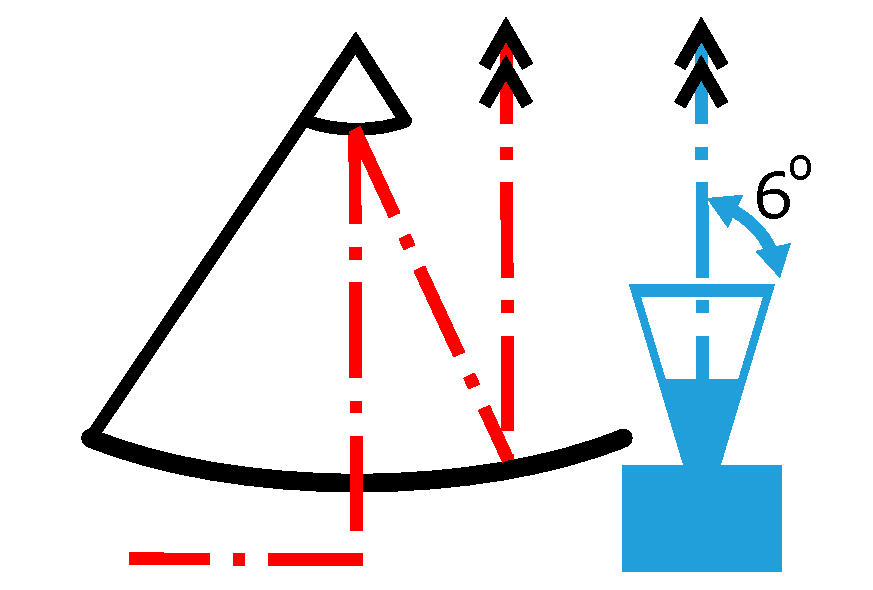
\includegraphics[width=0.45\linewidth]{figure2of4.eps}\label{fig:advanced2}}   
  \caption{Potential optical-communication configurations~\cite{Aretskin2019} showing star tracker and primary and secondary mirrors in a Cassegrain configuration: (\ref{fig:baseline2}) Baseline iROC co-boresight system with standard star tracker. (\ref{fig:advanced2}) Co-boresight with advanced star tracker. Note: Editing does want us to describe each sub-figure in this caption.}
  \label{fig:star_tracker}
\end{figure}

\begin{sidewaysfigure}[bth]
  \centering
  \includegraphics[width=.95\textwidth]{optical_com_2.png} \\
  \caption{\raggedright{Sometimes everything is more clear when a figure is put sideways and allowed to take up the whole page. This might make the figure get kicked to the end of the document and that is alright. Optical communication is fascinating. I have always wanted to try shining a laser from Mars to Earth.}}
  \label{fig:optical_com}
\end{sidewaysfigure}

% ============================================================================================
\subsection{Citations / Bibliography / References}
\label{sec:citations}
The bibliography is managed in a separate file which is surprisingly called \emph{bibliography.bib}. By editing this file you'll be able to add entries of your own. Once you are done you can reference them like I did here~\cite{Aretskin2019}. Reference your own work as often helps to increase it's apparent importance.



% ============================================================================================
% ============================================================================================
\section{Results}
\label{sec:results}
Your work has results right? Here is a great place to put them. Please remember not to send them out to the general public until your co-authors, peers, branch chief, project manager, export control, and editing department have all given you conflicting advice on how to change the document to meet their exacting expectations. 
%You might want to remind them you write it using a standard NASA \ac{TM} \LaTeX ~formatting document and maybe they will give you less grief. 




% ============================================================================================
% ============================================================================================

\acresetall         % Force reset of all acronyms (from intro and list) so that we can list them again in the conclusion.
\section{Conclusion} 
\label{sec:Conclusion}
Finally we made it to the end of the document. Now we need give the reader, who's brain is now irrevocably scrambled, a quick summary of the life-altering experience they just endured. We talked about general guidelines on writing style and we trained you on how to make subsections, equations, figures. You even have a nifty acronym handler that even works in the \ac{TM} conclusion. We showed you how to make tables and lists. 
Now we get to the part that I do not promise to perform any follow-on work since we never know what projects will have funding in 6 months.
As a final reminder, if you want this template to be fixed, you can do it yourself by submitting change requests on GitHub\footnote{\url{https://github.com/ehariton/TM_template}}.



\end{flushleft} % we need this here don't delete me


%% ----------------------------------------------------------------------------------------------------------------------------------
%% 										 BIBLIOGRAPHY
%% ----------------------------------------------------------------------------------------------------------------------------------
\begingroup
\raggedright
\bibliography{bibliography.bib}
\endgroup



\end{document}
